\documentclass[main]{subfiles}
\begin{document}

%@@@@@@@@@@@@@@@@@@@@@@@@@@@@@@
% Main Topics: Action Potential 18.10.2018
% Lecturer: Valerio Mante
% author: Vanessa Leite - base document from benelot/eth-intro-to-neuroinformatics-summary

\section{Action Potential (AP)}
\begin{itemize}[noitemsep,nolistsep]
	\item Occurs in \textbf{axons}
	\item \textbf{All-or-none}, i.e., stereotyped (if $I_e$ increases it will lead to an AP initiated sooner, but with the same shape. It is non linear, unlike passive membrane).
	\item It travels down the axon (if initiated close to the soma, i.e., in axon initial segment).
	\item Hodgkin-Huxley: Nobel Prize Medicine Physiology in 1963. Everything they did was before the existence of ion-channel was known.
	\item Refraction period ensures maximum frequency.
	\item Action potential is about $1$ to $10\,m/s$ fast.
	\item It would take 100 years to go through all axons of the human brain in a serial fashion.
\end{itemize}

\begin{figure}[H]
	\centering
	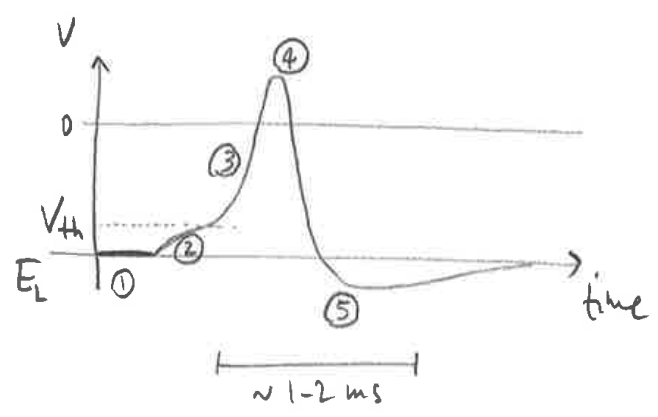
\includegraphics[width=0.5\textwidth]{action-potential-01.png}
	\caption{\textbf{1}: at rest, $V=E_L$ (resting potential); \textbf{2}: current injected ($I_e$) leads to an increase in $V$ exponentially, for small $I_e$ it doesnt reach $V_{th}$. Large $I_e$ crosses $V_{th}$; \textbf{3} If $V > V_{th}$ a fast depolarization happens, i.e., an AP; \textbf{4} overshoot $V > 0$ (around $30mV$); \textbf{5}: hyperpolarization and undershoot ($V < E_L$).}
\end{figure}

During an AP we see channels opening and pulling $V$ towards $E$. 
The hypotheses is that in the rising phase of AP the sodium and calcium conductances increase ($g_{Na}$ and $g_{Ca}$), and in the decaying phase of AP the sodium and calcium conductances decrease or potassium and chloride conductances increase. All as function of $V$.
For testing this hypotheses, we need to measure $g_{Na}, g_K$ etc. We can use the $IV$-relation: measuring $I_{Na}, I_K$ etc for different $V$ then infer $g_{Na}, g_K$, etc. To do this, we can use voltage clamp.

\subsection{Voltage clamp}
A new technique invented by Hodgkin and Huxley. Previously, current $I_e$ was injected and voltage $V$ was measured, now set $V$ and measure $I_e$ required  to keep $V_{measured} = V_{set}$.
It measures the current required to clamp the membrane voltage. Fast feedback system to fix $V$ and measure $I$.

$I_e$ has opposit sign, i.e., is positive if from outside to inside. But to keep the $\Delta V$ constant, it is necessary to inject a current opposite to the ionic current. In the end, the current injected can be read as the ionic current (in the ionic current convention).

\paragraph{Space clamp} Makes the axon isopotential, do not have an AP but it is the same mechanism.

The giant axon in squid has approximately $1mm$ of diameter and it is like a long wire, making the axon isopotential.

\subsubsection{Voltage clamp experiment}

\begin{figure}[H]
	\centering
	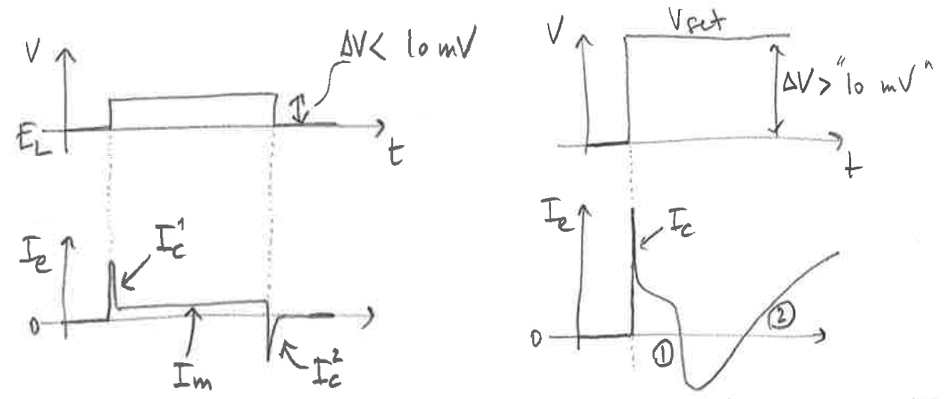
\includegraphics[width=0.8\textwidth]{voltage-clamp-experiment.png}
	\caption{On left, small voltage is applied: passive/linear membrane. $I_c^1$ depolarizes membrane (add $+$ charge to inside). $I_m$ compensates for leak current $I_L$ ($V \neq E_L$: cell wants to go bad to $E_L$). $I_c^2$ repolarize the membrane, i.e., remove charged added in $I_c^1$; On right, large $V$ is applied ($V > 10 mV$, i.e.,$V > V_{th}$: active, non linear membrane. In \textbf{1} cell wants to depolarize, there is a need to inject negative $I_e$ to keep $V = V_{set}$. $I_{Na}$, $E_{Na} \approx 50mV$; In \textbf{2} cell wants to hyperpolarize, there is a need to inject positive $I_e$ to keep $V = V_{set}$. $I_K$, $E_K \approx -80mV$.}
\end{figure}

\begin{itemize}[noitemsep,nolistsep]
	\item Command voltage is set by the experimenter, the feedback circuit holds the voltage constant.
	\item The voltage clamp allows the membrane voltage to be manipulated independently of ionic currents, allowing the current-voltage relationships of membrane channels to be studied.
	\item With negative feedback circuit, the $Na^+$ current is auto-catalytic. An increase in the voltage increases conductance, which increases the $Na^+$ current, which increases the voltage again.
	\item The threshold for action potential initiation is where the inward $Na^+$ current exactly balances the outward $K^+$ current.
\end{itemize}

\begin{figure}[H]
	\centering
	\begin{subfigure}[b]{0.5\textwidth}
    	\centering
		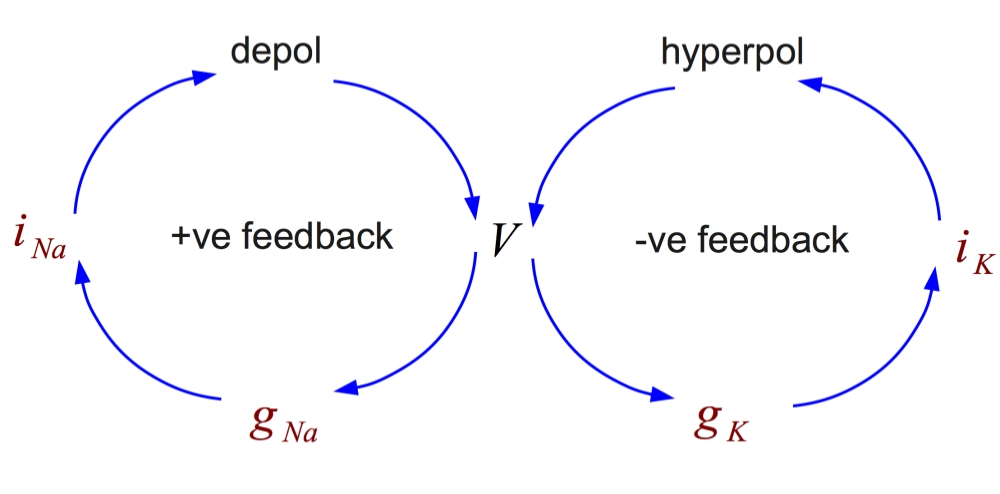
\includegraphics[width=\textwidth]{5_7.jpg}
	\end{subfigure}%
	~
	\begin{subfigure}[b]{0.4\textwidth}
		\centering
		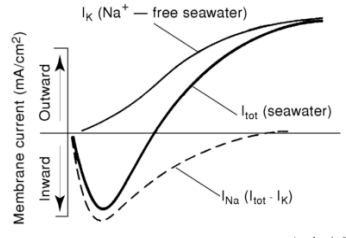
\includegraphics[width=\textwidth]{voltage_clamp_01.png}
	\end{subfigure}
\end{figure}

\subsubsection{Identifying the nature of the current}

\paragraph{H and H: remove $Na$ gradients}
They replaced extracelullar medium with a solution that has $10\% Na^+ $ compared to seawater. This eliminates $I_{Na}$ for $\Delta V \approx 50 mV $  ($[Na]_{in} = [Na]_{ou}$).
By repeating the experiment for many $V_{set}$ (i.e., $\Delta V$) they get $I_{Na}(V)$ and $I_K(V)$.
$I_{Na} = I_{seawater} - I_K$.
get $g_{Na}(V)$ and $g_K(V)$ with $I_{Na} = g_{Na}(V - E_{Na})$ and $I_K = g_K (V - E_K)$.

\paragraph{Later: removed intracelullar $K^+$} It confirmed $I_K$ and H and H predictions.

\paragraph{Pharmacology} Uses pharmacological blockages.
\subparagraph{TTX} poison in pufferfish, it eliminates $I_{Na}$.
\subparagraph{TEA} eliminates $I_K$.

\begin{figure}[H]
	\centering
	\begin{subfigure}[b]{0.65\textwidth}
    	\centering
		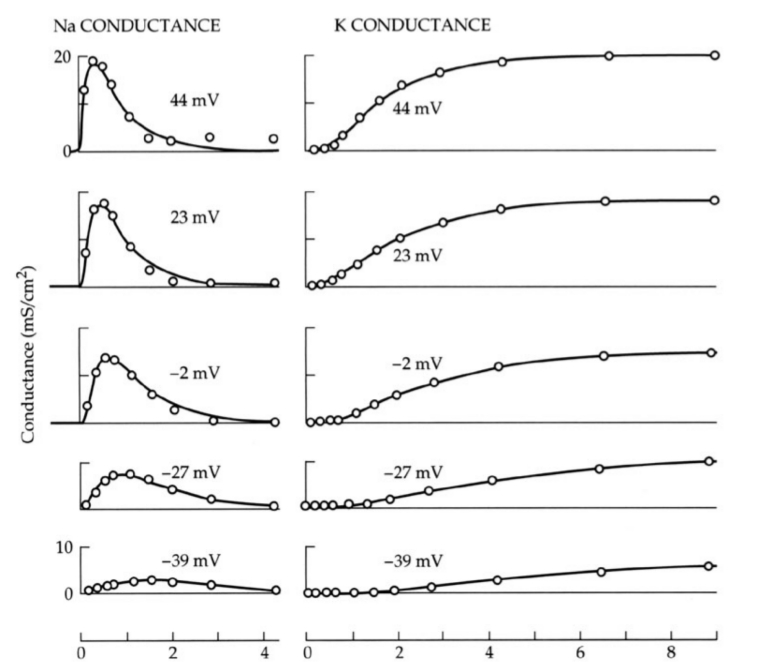
\includegraphics[width=\textwidth]{5_4.jpg}
	\end{subfigure}%
	~
	\begin{subfigure}[b]{0.35\textwidth}
		\centering
		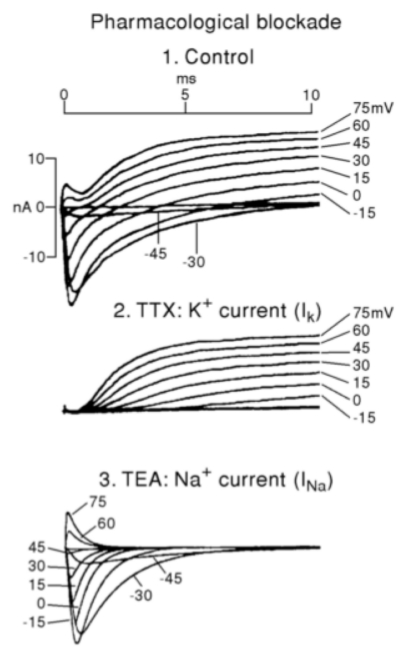
\includegraphics[width=\textwidth]{5_4_2.jpg}
	\end{subfigure}
\end{figure}

Voltage and time dependent conductances for $g_{Na}, g_{K}$: 
$g_{Na}$ increases quickly (fast activation), but then inactivation kicks in and it decreases again (fast inactivation).
$g_K$ increases more slowly (slow activation), and only decreases once the voltage has decreased (no inactivation).

\subsubsection{Voltage and time dependent conductances}
Two possibilities that cause conductance to be voltage and time dependent:
\begin{enumerate}
\item Single channels have variable permeability (analog)
\item Single channels are either opened or closed (digital)
\subitem today we know, this is the correct option
\end{enumerate}

\subsection{Patch clamp}
\begin{itemize}
\item Technique that allows recording of current $I$ through a single channel
\item Neher and Sakmann - Nobel prize in Medicine and Physiology in 1991
\item H and H inferred it from their Voltage clamp data
\item Individual channels are probabilistic devices that are opened or closed. The conductance is measured by the average of all channels.
\end{itemize}

There are two types of voltage-dependent conductances:
\paragraph{Persistent conductance type} It has two stages: deactivated (closed) and activated (opened). The channel opens and stay opened when the cell is depolarized. For example, $g_K$ in AP.
\paragraph{Transient conductance type} It has three stages: deactivated, activated and inactivated. Here we have two gating variables that describe the opening and closing of the channel. Activation and Inactivation are two process that work in opposite directions. The channel opens but then it closes while the cell  is still depolarized. For example, $g_{Na}$ in AP.

\paragraph{H and H formalism} It is used for active conductances in general.
\[g_i = \bar{g_i} \cdot P_i \] where $g_i$ is the overall conductance of channels of type $i$; $\bar{g_i}$ is the maximal conductance (if all the channels were open); and $P_i$ is the probability of the channel be open (or the fraction of channels that are open).

\subsubsection{Persistent conductance}
Assume that $k$ events (independents and identical) are necessary to open a single channel, then $P = n^k$.
$n$ is a gating/activation variable: the probability of a subunit gate being open, and it is voltage and time dependent.
$k$ is the number of subunits necessary to open each channel.

\paragraph{H and H} $g_K = \bar{g_K} \cdot P_K \rightarrow P_K = n^4 = n \cdot n \cdot n \cdot n$ (it is necessary $4$ subunits to open the channel).
When $k$ was fitted to data it leaded to corrected predictions for $K^+$ channels.

\paragraph{Time dependence}

Assume closed $\rightarrow$ opened and opened $\rightarrow$ closed transitions such that:
\[\underbrace{\Delta n}_\text{change in the number of open channels in time t} = \underbrace{\alpha_n (V)}_\text{rate of opening} \cdot \underbrace{(1-n)}_\text{fraction of closed} \cdot \underbrace{\Delta t}_\text{time} - \underbrace{\beta_n (V)}_\text{rate of closing} \cdot \underbrace{n}_\text{fraction of opened} \cdot \Delta t \]

If channels closed $\rightarrow$ open, then $\Delta n > 0$, open $\rightarrow$ closed, then $\Delta n < 0$.

At $\Delta t = 0$, $\frac{dn}{dt} = \alpha_n (V) (1 - n(t)) - \beta_n (V) n(t)$, $\alpha_n$ and $\beta_n$ are not time dependent.

$\rightarrow \tau_n(V) \cdot \frac{dn}{dt} = n_\infty(V) - n$,
where $\tau_n(V) = \frac{1}{\alpha_n(V) + \beta_n(V)}$ and $n_\infty(V) = \frac{\alpha_n(V)}{\alpha_n(V) + \beta_n(V)}$. $0 \leq n_\infty(V) \geq 1$.

For $\tau_n(V)$ we have that faster transitions leads to faster change in $n$.

\begin{figure}[H]
	\centering
	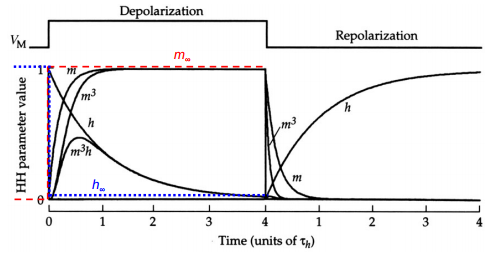
\includegraphics[scale=1.0]{depolarization_01.png}
	\caption{Gating variables: time dependence}
\end{figure} 

\paragraph{Voltage dependence}
How to determine the values of $\alpha_n(V)$ and $\beta_n(V)$?
In practice: $\alpha_n(V)$ and $\beta_n(V)$ are fitted to data (i.e., $g_K(V,t)$).
$\alpha_n(V)$ and $\beta_n(V)$ are approximately exponential because the energy barriers that need to be overcome by the gating change.

In this case, $\alpha_n(V) \approx A_\alpha \cdot e^{-\frac{E_\alpha}{k_B T}}$ and $\beta_n(V) \approx A_\beta \cdot e^{-\frac{E_\beta}{k_B T}}$

\begin{figure}[H]
	\centering
	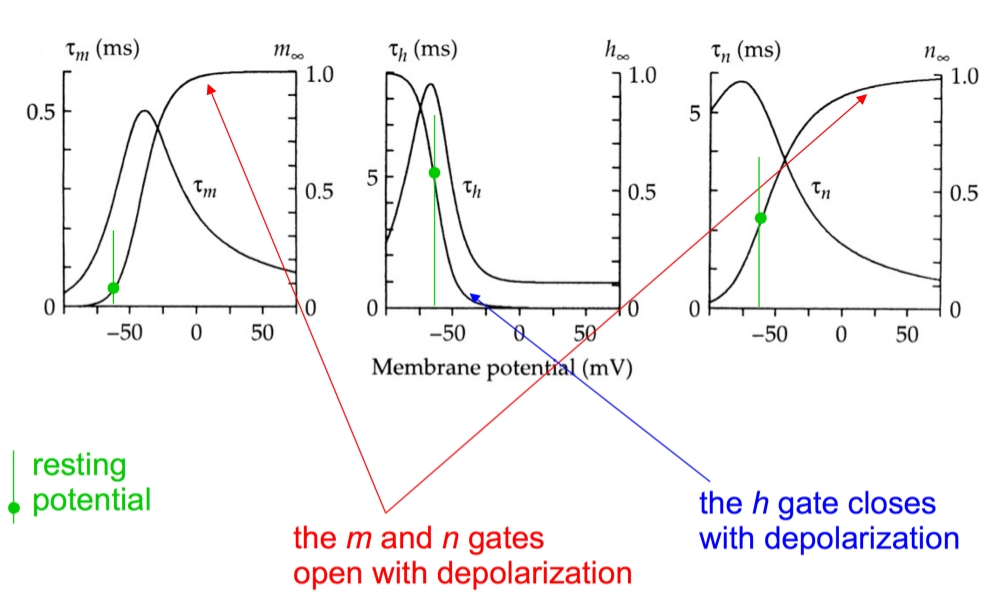
\includegraphics[scale=0.5]{5_8.jpg}
	\caption{Gating variable: voltage dependence}
\end{figure} 

\subsubsection{Transient conductance}
Similar, but includes inactivation: $P_{Na} = \underbrace{m^3}_\text{activation variable} \cdot \underbrace{h}_\text{inactivation variable}$.
$h$ is the probability that channel is not blocked by inactivation gate.

\begin{figure}[H]
	\centering
	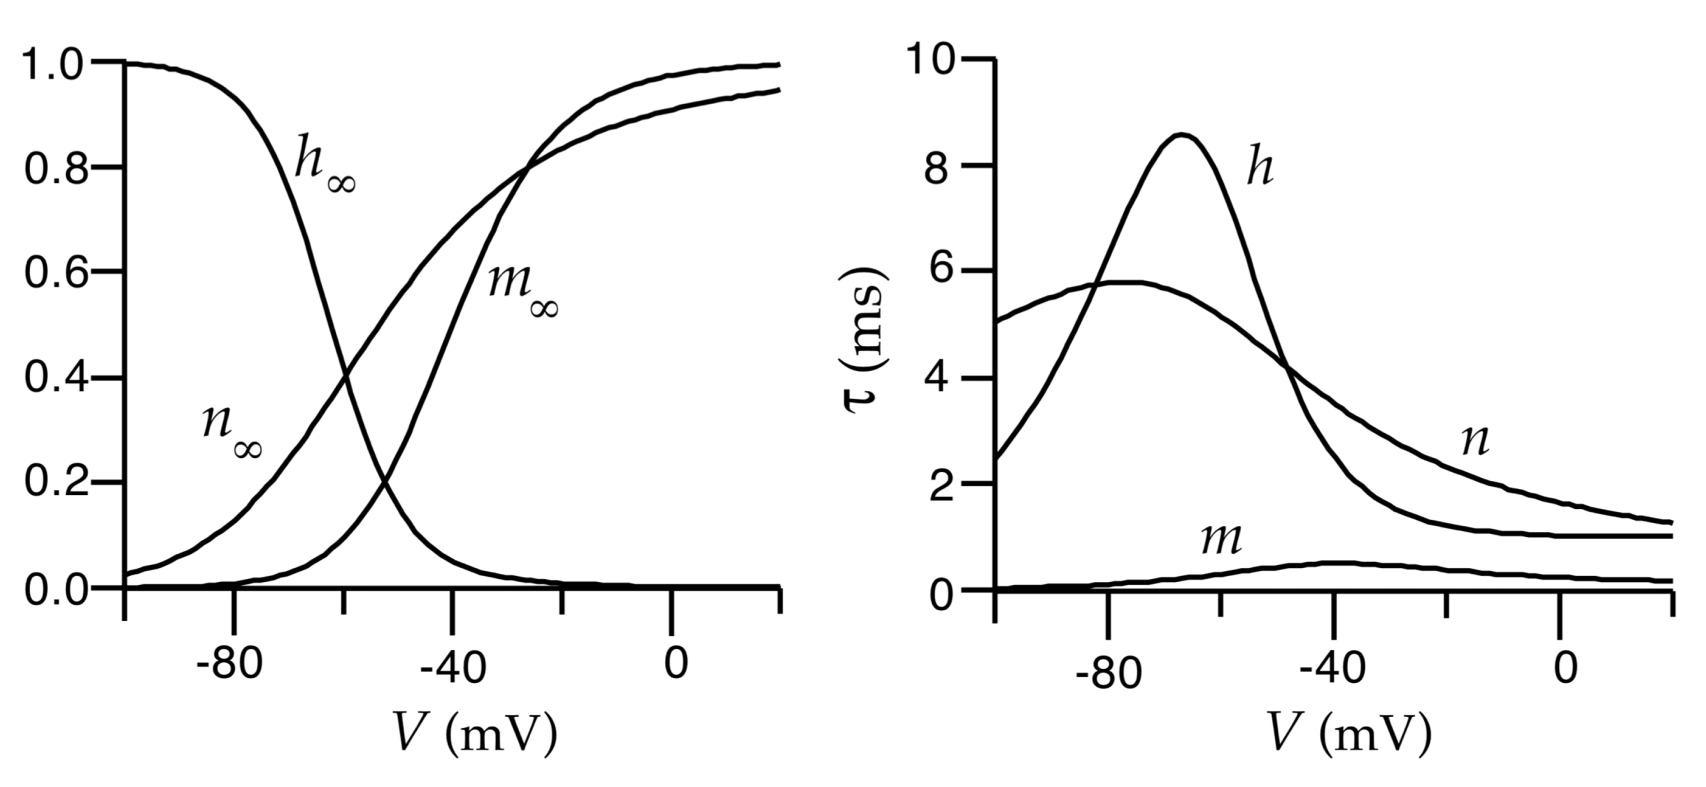
\includegraphics[width=0.5\textwidth]{gating-dependence.png}
	\caption{$m$ is fast, $h$ and $n$ are slow. $m$ and $h$ have opposite $V$-dependence.}
\end{figure} 

\subsection{Full Hodgkin-Huxley Model}

\begin{figure}[H]
	\centering
	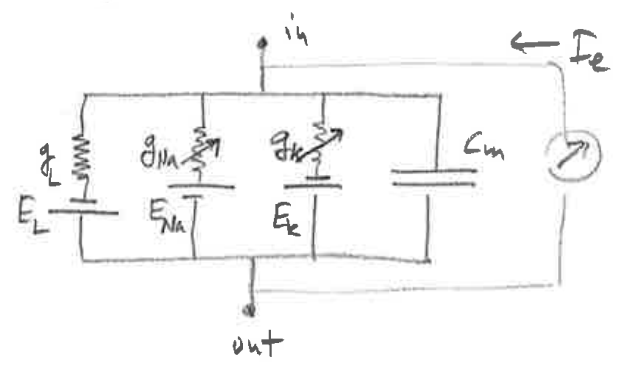
\includegraphics[width=0.5\textwidth]{full-HH-model.png}
\end{figure} 

\begin{itemize}
	\item Model that describes how action potentials in neurons are initiated and propagated.
	\subitem model parameters are fit to $g_{Na}(V,t)$ and $g_K(V,t)$ from voltage clamp.
	\item $n$ and $m$ are probabilities for a gate to be open.
	\item $h$ is the probability that an open channel is not blocked.
	\item The gating variables have a voltage dependence.
	\item $\bar{g}$ values are the maximum conductance possible.
	\item There is no inactivation for potassium, only for sodium.
	\item The membrane does not get locked at positive values.
	\item $\bar{g}_L$ stands for some generic leak.
	\item The functions $n_\infty(V)$, $m_\infty(V)$ and $h_\infty(V)$ determine whether gates serve to activate channels (with depolarization) or inactivate the channel (close with depolarization). $\tau_m$, $\tau_h$ and $\tau_n$ are time constants.
\end{itemize}

\[C\frac{dV}{dt}+\bar{g}_Kn^4(V-V_K)+\bar{g}_{Na}m^3h(V-V_{Na})+\bar{g}_L(V-V_L)+I_{inj}=0\]

\paragraph{Some model parameters}
$\bar{g_L} = 0.003 mS/mm^2$, $E_L = -54mV$\\
$\bar{g_K} = 0.036 mS/mm^2$, $E_K = -77mV$\\
$\bar{g_{Na}} = 1.2 mS/mm^2$, $E_{Na} = +50mV$\\
here, $S$ stands for Siemens = $\frac{1}{ohm}$

\paragraph{Model predictions}
\subparagraph{AP-shape}

\subparagraph{AP-threshold}
$n_\infty$, $m_\infty$ and $h_\infty$ are all $> 0$ for $V = E_L (= V_{rest})$.
That means that $g_{Na}$ is already open at rest.
Why we have no AP at rest? $I_L$ and $I_K$ are larger than $I_{Na}$ for $V < V_{th}$. At $V_{th}: |I_L + I_{K}| = |I_{Na}|$.

\subparagraph{Refractory period}
It is harder (requires larger current injection) to generate AP immediately after an AP. The reason is that $g_K$ is still activated and $g_{Na}$ is still inactivated.

\subparagraph{AP propagation in unmyelinated axon}

\subparagraph{AP propagation in myelinated axon}
In the myelinated part of the axon we have passive AP propation (small capacitance and large resistance), but in the nodes of ranvier, we have active AP regeneration.
Compared to unmyelinated:
\begin{itemize}
\item faster AP propagation
\item smaller current
\item faster $V_{AP}$ increase with axon radius
\end{itemize}

\subparagraph{AP propagates in one direction along axon}
Reason: refractory period, $g_{Na}$ still inactivated  in the wake of AP. Either direction is possible in principle. From soma to axon terminal: orthodromic. In the opposite direction: antidromic. In the brain we do not have usually antidromic AP.
Antidromic AP can be generated artificially. With a collision experiment, i.e., both antidromic and orthodromic AP initiated, none achieve the other end, they annihilate each other.

\subparagraph{AP not reflected at axon terminal}
At the end of the cable, there is no AP reflected because refractory period.

\subparagraph{AP does not usually propagate in dendrites}
Because $g_{Na}$ is missing. However, in a few cell types $g_{Na}$ is present also in dendrites. It is not sufficient to generate an AP, but can propagate AP from soma into dendrite to some extent: axon backpropagation.

\subparagraph{Number of subunits in $K$ channel}
It was verified much later with structural studies.

%\subsection{Equilibrium voltage}
%\begin{itemize}[noitemsep,nolistsep]
%	\item When $I_m = 0$ and $\frac{dv}{dt}=0$ then
%	\item $V=\frac{g_KE_K+g_{Na}E_{Na}+g_{Cl}E_{Cl}}{g_K+g_{Na}+g_{Cl}}$
%	\item $I_m = I_{cap}+I_K+I_{Na}+I_{L}$
%\end{itemize}

\end{document}
